\documentclass[12pt,a4paper]{article}

%\usepackage{german}
\usepackage{a4wide}
\usepackage{graphicx}
\usepackage{amssymb}
\usepackage{amsmath}
%\usepackage{ae,aecompl}

\pagestyle{empty}
\setlength{\parindent}{0pt}
\renewcommand{\labelenumi}{\alph{enumi})}
\renewcommand{\labelenumii}{\roman{enumii})}

\newcommand{\aufg}[1]{\vspace{4mm}{\bf\underline{Problem #1:}}\vspace{3mm}}

\begin{document}
\vspace*{-3cm}
\begin{center}
{\large\bf GLoBES Tutorial: Using user-defined systematics and
  oscillation probabilities}\\[0.3cm]
GLoBES workshop in Heidelberg, Germany, January 24-26, 2007
\end{center}
\vspace*{2mm}

Patrick\ Huber \hfill \today

\bigskip
\hrule
\vspace*{4mm}

{\small In this advanced-level tutorial, we show how to use
  user-defined $\chi^2$-functions to treat a two detector setup with
  various systematical errors. This configuration is relevant for
  reactor neutrino experiments like Double Chooz.
  
  In a second part we will provide an example of how define an
  oscillation probability engine which includes non-standard physics.
  In the case at hand we deal with some form of 'decoherence' which
  leads to an exponential damping of the oscillation signature.  }

\vspace*{0.5cm}

\subsection*{Part 1: Reactor neutrino experiments}

In a reactor neutrino experiment, one tries to determine
$\sin^22\theta_{13}$ by measuring the disappearance of $\bar\nu_e$. In
order to be able to measure this small effect it is crucial to know
how many neutrinos are emitted from the source. To this end a near
detector is used. The comparison of event rates between near and far
detector allows to cancel most of the systematics associated with
source and only the relative normalization of the two detectors remains
(at first order). This setup cannot be described within GLoBES without
using a special user-defined $\chi^2$-function. The example shown here
is taken from~\cite{Huber:2006vr} and quite accurately describes
Double Chooz.

The actual C-code is in {\tt systematic.c}, typing {\tt make} should
compile the software and {\tt ./systenatic} executes the program,
which takes about 1 minute to finish. It will produce four data files
{\tt sys-data0} till {\tt sys-data3}. You can use {\tt gnuplot <
  systematic.gnuplot} to produce a plot, {\tt systematic.eps}. We use
{\tt gnuplot} in this example because it is GPL'd and widely
available, but of course, you can use whatever software you prefer for
plotting. In some cases you might want to adjust the output format to
fit your preference.


\aufg{1} {\bf The AEDL files}

First, we need to have a description of the two detectors. Have a look
a {\tt D-Chooz\_far.glb} and {\tt D-Chooz\_near.glb}. What are the
differences beyond the obvious baseline?

\begin{enumerate}
\item {\tt @norm} -- the near detector is less efficient, basically
  because it has less overburden, hence higher backgrounds and thus
  less life time.
\item {\tt @sys\_on\_function} -- {\tt chiZero} is used for the near
  detector since we want to compute the $\chi^2$ only once.
  Otherwise GLoBES would compute it for each detector since they are
  regarded as two experiments. {\tt
    chiDCNorm} is used for the far detector and describes a $\chi^2$
  definition which includes an error on the flux, the fiducial mass of
  the near detector, the fiducial mass of the far detector, the energy
  scale of the near detector and the energy scale of the far detector.
The definition of the $\chi^2$ is
\begin{align}
  \chi^2 &= \chi^2_{F} + \chi^2_{N} + \chi^2_\mathrm{pull}
\, ,
  \label{eq:chi2total}
\end{align}

where
\begin{align}
  \hspace{-1 cm} \chi^2_{F} &= \sum_i
     \frac{\left[ (1 + a_{F,\rm fid} + a_{\rm norm} ) T_{
F,i}\, - O_{F,i} \right]^2}{O_{F,i}} \, , \label{eq:chi2F1} \\
  \hspace{-1 cm} \chi^2_{N} &= \sum_i
    \frac{\left[ (1 + a_{N,\rm fid} + a_{\rm norm}) T_{N,i
}
        - O_{N,i} \right]^2}{O_{N,i}}     \, ,    \label{eq:chi2N2} \\
  \hspace{-1 cm} \chi^2_\mathrm{pull} &= \frac{a_{F,\rm fid}^2}{\sigma_{F,\rm fi
d}^2}
       \, +\, \frac{a_{N,\rm fid}^2}{\sigma_{N,\rm fid}^2}
       \, +\, \frac{a_{\rm norm}^2}{\sigma_{\rm norm}^2} \, .
       \label{eq:chi2pull}
\end{align}

Finally, we introduce an energy calibration error which is implemented
as a re-binning of $T_{F,i}$, and $T_{N,i}$ before
the $\chi^2$ analysis (see App.~A of~\cite{Huber:2003pm}). It is uncorrelated
between the two detectors.

\item {\tt @sys\_on\_errors} -- of course contains only values if {\tt
    chiDCNorm} is used.
\end{enumerate}

\aufg{2} {\bf The $\mathbf{\chi}^2$-function}

Now that we have the AEDL files, we need to define the $\chi^2$-function
and have to make sure that GLoBES knows about it. It is quite
straightforward to write code which realizes above definition.

There are two things in the definition of {\tt chiDCNorm}, which need
to be mentioned: For implementing the energy scale error we use the
GLoBES function {\tt  glbShiftEnergyScale}. Second, in order to ensure
good performance we just get the memory address from GLoBES where is
stores all its event rates (pass by reference). This address does not
change during the computation and therefore our own $\chi^2$-function
is as effective as the GLoBES built-ins. The functions used for that
is {\tt  glbGetRuleRatePtr}.

The new $\chi^2$-function has to be registered. This serves a
two-fold purpose: GLoBES needs to know what function to actually use
and secondly, in that process you give  your new
function a name. This name will be used in the AEDL file to identify your
function and thus prevents errors from using the wrong function.
 
\aufg{3} {\bf Adding a shape error}

So far, we have no way to account for the fact the neutrino spectrum
of  a nuclear reactor is only known up to some accuracy. There are two
reasons for that: the neutrinos are produced by a mixture of isotopes
and this mixture initially is only known with some error and moreover
changes during reactor operation (burn-up). The other reason is that
the neutrino spectrum for each isotope is measured only with some
accuracy. We lump all these effects together in what is called a shape
error. Basically, this is an error which changes the number of events
in a bin uncorrelated with any other bin, but fully correlated between
detectors. This error largely cancels in a two detector setup.
\begin{align}
  \hspace{-1cm} \chi^2_{F} &= \sum_i
     \frac{\left[ (1 + a_{F,\rm fid} + a_{\rm norm} + a_{\mathrm{shape}, i}) T_{F,i}
        - O_{F,i} \right]^2}{O_{F,i}}      \, ,    \\
  \hspace{-1 cm} \chi^2_{N} &= \sum_i
    \frac{\left[ (1 + a_{N,\rm fid} + a_{\rm norm}+ a_{\mathrm{shape},i}) T_{N,i}
       - O_{N,i} \right]^2}{O_{N,i}}     \, ,    \ \\
  \hspace{-1 cm} \chi^2_\mathrm{pull} &= \frac{a_{F,\rm fid}^2}{\sigma_{F,\rm fid}^2}
       \, +\, \frac{a_{N,\rm fid}^2}{\sigma_{N,\rm fid}^2}
       \, +\, \frac{a_{\rm norm}^2}{\sigma_{\rm norm}^2}
       \, +\, \sum_i \frac{a_{\mathrm{shape},i}^2}{\sigma_{\mathrm{shape},i}^2}\, .      
\end{align}
This definition increases the number of nuisance parameters quite a
lot and that creates some issues with the convergence of the numerical
minimization. This can be alleviated by a clever way to chose the
starting values for this minimization. We always will start with a
very small $\sin^22\theta_{13}$ and save the location of the minimum.
We use that as starting value for the next larger value of
$\sin^22\theta_{13}$. If the step size in $\sin^22\theta_{13}$ is
small enough we get good convergence. Just try setting {\tt
  step\_size} to $0.1$ (instead of $0.01$) and you will see that
introducing the shape error makes the $\chi^2$ larger! This is a clear
sign of failure to converge.

\aufg{4} {\bf Adding a bin-to-bin error}

A bin-to-bin error is a theorist's way to account for all those little
real world things which you only know once you have done the
experiment. It is like a shape error but now also uncorrelated between
near and far detector. That is the $a_{\mathrm{shape},i}$ acquire one more
index and there are twice as many. 

\begin{center}
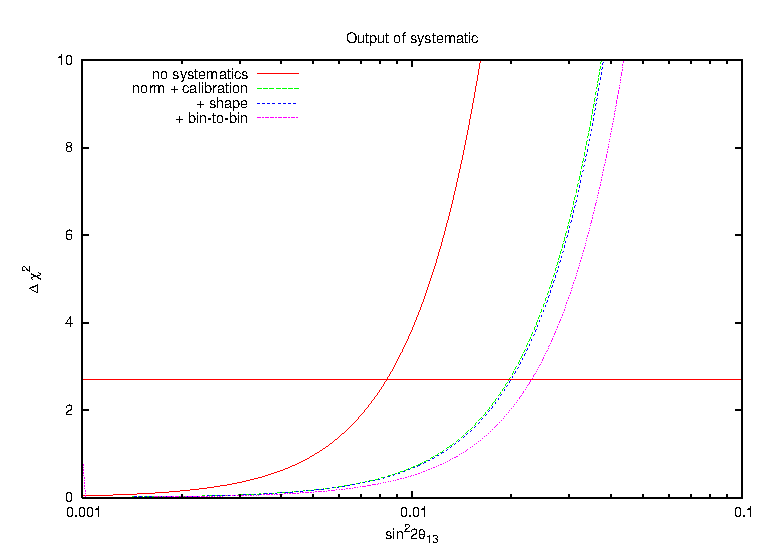
\includegraphics[width=0.8\textwidth]{systematic}
\end{center}

\subsection*{Part 2: Non-standard physics}

In principle one can imagine an arbitrary number of non-standard
scenarios, like 4 neutrinos, modified matter effect,
Lorentz-invariance violation asf. GLoBES now allows the user to supply
his own oscillation probability routines. This feature is not only
useful to deal with non-standard effects, but it can be used to write
debugging  tools (like watching the minimizers step-by-step) or to
provide routines which are optimized for a certain application.

Here we will discuss a so called damping effect in a reactor neutrino
experiment. The reactor experiment will be much simpler than in the
previous section and consists only of one detector. The oscillation
physics is taken from~\cite{Blennow:2005yk}.

The actual C-code is in {\tt oscillation.c}, typing {\tt make} should
compile the software and {\tt ./oscillation} executes the program,
which takes about 1 minute to finish. It will produce two data files
{\tt osc-data1} and {\tt osc-data2}. You can use {\tt gnuplot <
  oscillation.gnuplot} to produce a plot, {\tt oscillation.eps}.


\aufg{1} {\bf Implementing the oscillation engine}

The oscillation probability for our example is given by

\begin{eqnarray}
P_{\bar e\bar e} &=&
c_{13}^4 \left\{ 1-2 s_{12}^2 c_{12}^2 ( 1-D_{21}\cos(2\Delta_{21}))
  \right\}\nonumber\\
&&+2 s_{13}^2 c_{13}^2 [D_{21} c_{12}^2 \cos(2\Delta_{31})\nonumber\\
&&+D_{32}s_{12}^2\cos(2\Delta_{32})] + s_{13}^2 
\,,
\end{eqnarray}

where 

\begin{equation}
D_{ij}=\exp \left[ -4 \left(\Delta_{ij} \frac{\sigma_E}{E}\right)^2\right]\,.
\end{equation}
Thus we have one additional parameter $\sigma_E$ which has unit GeV.

\aufg{2} {\bf Using the new parameter}

Once we have an oscillation routine which can handle non-standard
physics, we have to maintain this new parameter and understand how the
minimizer deals with additional parameters.

\begin{center}
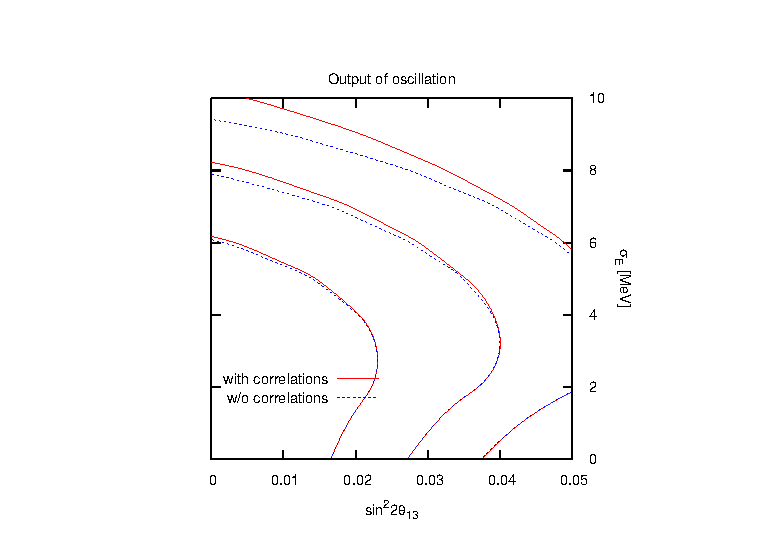
\includegraphics[width=0.8\textwidth]{oscillation}
\end{center}

\bibliographystyle{./apsrev}
\bibliography{references}

\end{document}
